\section{Ähnliche Ansätze}\label{schliecker}
Bedürfnisbasierte Agenten kommen in verschiedenen Spielen zum Einsatz. Recherchen legen allerdings die Vermutung nahe, dass es bisher keine Beispiele für die Nutzung von Reinforcement Learning in Kombination mit bedürfnisbasierten Agenten gibt. Es konnte allerdings eine Bachelorarbeit mit dem Titel \Fachbegriff{Verhaltenssteuerung bedürfnisorientierter NPCs in Rollenspielen mithilfe Neuronaler Netze} gefunden werden, in der überwachtes Lernen genutzt wurde \cite{dorf_agents_kevin}. Der Lernvorgang wurde ebenfalls genutzt, um den Agenten beizubringen, Entscheidungen aufgrund ihrer Bedürfnisse zu treffen. In der Arbeit wird die Bedürfnistheorie nach Maslov berücksichtigt, um den Agenten ein möglichst menschliches Verhalten zu verleihen \cite{maslov_needs}. Für den Lernprozess wurden auf der Grundlage von Formeln, die von Maslov aufgestellt wurden, Trainingsdaten generiert.




\section{Vergleich der Ansätze}
Im Folgenden werden die drei entwickelten Ansätze im Bezug auf den Entwicklungsaufwand und das resultierende Verhalten der Agenten untersucht und verglichen. Alle Verfahren beruhen auf derselben zugrunde liegenden Architektur der Dorfsimulation. Sie unterscheiden sich lediglich in der Art und Weise, wie die Agenten Entscheidungen fällen, um Aktionen auszuführen. Die Analyse bezieht sich nicht auf die Architektur der gesamten Dorfsimulation, sondern nur auf den jeweiligen Entscheidungsprozess und der jeweils damit verbundenen Implementierung.

\subsection{Benötigter Entwicklungsaufwand}
Im Folgenden wird der nötige Entwicklungsaufwand für die Implementierungen der einzelnen Ansätze betrachtet.


\subsubsection{GOAP}
Die GOAP-Implementierung benötigte einen höheren Entwicklungsaufwand, da bestehende ActionPlans nicht genutzt werden konnten. Diese Änderungen waren notwendig, weil GOAP und die verwendete Bibliothek für die Ausführung von Aktionen eine andere Architektur erwarten. 

Ein großes Problem war dabei die Definition von Effekten und Bedingungen für GoapActions. Für das Erreichen eines Ziels werden bei GOAP einzelne Aktionen ausgeführt, die essentiell sind - für einen Bäcker beispielsweise \Fachbegriff{Hole Mehl} oder \Fachbegriff{Backe Brot}. Die für die anderen Ansätze verwendeten ActionPlans definieren ganze Sequenzen von Aktionen, die zusammen eine größere Aktion beschreiben. Solche Sequenzen können durch GOAP nicht beschrieben werden, da einzelne Aktionen dort jeweils genau einen Zielort haben und die Auswahl der elementaren Aktionen vollständig durch die Bibliothek übernommen wird. Zum Beispiel werden im ActionPlan \inlinecode{WorkBakeryActionPlan} sequentielle Teilaktionen definiert, sodass der Agent erst zur Bäckerei, dann zum Hauptlager, dann wieder zur Bäckerei und schließlich wieder zurück zum Hauptlager geht. Dadurch soll auf sehr einfache Weise simuliert werden, dass der Bäcker Mehl aus dem Lager holt (vorhandes Mehl ist eine Voraussetzung für die Ausführung der Aktion), dann Brot backt und schließlich das fertige Brot in das Lager bringt. Wenn man diesen Vorgang in GOAP modellieren möchte, muss eine große Menge von Effekten und Bedingungen eingeführt werden. Zunächst braucht der Bäcker entweder ein eigenes Inventar und für jede Ressource einen Effekt \Fachbegriff{HAS\_RESOURCE} mit der jeweiligen Aktion \Fachbegriff{FETCH\_RESOURCE\_FROM\_STORAGE}. Für jede Ressource muss geprüft werden können, ob der Bäcker diese bereits in seinem Inventar besitzt. Falls dies nicht der Fall ist, muss die Ressource geholt werden. Anschließend benötigt man die Aktion \Fachbegriff{BAKE\_BREAD} mit einem Effekt \Fachbegriff{HAS\_BREAD} und einer weiteren Aktion \Fachbegriff{MOVE\_RESOURCE\_TO\_STORAGE}, um das Brot zum Lager zu bringen. 
In welcher Reihenfolge diese Aktionen ausgeführt werden, ist dabei nicht kontrollierbar. Insgesamt erreicht man schnell eine sehr hohe Anzahl von Effekten, Bedingungen und Aktionen. Diese hohe Anzahl ist dadurch bedingt, dass die Dorfsimulation nicht mit der Idee entwickelt wurde, GOAP zu verwenden. Ein weiteres Problem besteht darin, dass in der verwendeten Bibliothek für jede GoapAction stets nur ein Zielort definiert werden kann. Die Dorfsimulation baut aber darauf auf, dass Gebäude über bestimmte Kapazitäten verfügen und die Zielorte von Aktionen daher dynmaisch durch den \inlinecode{LocationHandler} definiert werden. GoapActions erwarten aber bereits bei der Initialisierung einen Zielort. Die entstandene Architektur eignet sich daher insgesamt wenig für die Anwendung von GOAP. Die GOAP-Bibliothek verwendet darüber hinaus die Bibliothek \cite{ninja} und beruht auf der asynchronen Ausführung von Coroutines. Wegen der Eigenheiten von GOAP und des verwendeten Multithreadings mussten zahlreiche Änderungen vorgenommen werden, um GOAP zu nutzen - beispielsweise im \inlinecode{LocationHandler}.

Konkret traten in der Bibliothek Fehler bei der Erzeugung der Aktionsbäume zum Erreichen von Zielen auf. Es wurden Änderungen im Programmcode der Bibliothek vorgenommen, sodass beispielsweise die Größe der entstandenen Bäume auf einen Maximalwert beschränkt wurden, was die Probleme nur teilweise lösen konnten. Tatsächlich entstanden dadurch im Gegenteil zusätzliche Probleme, da nicht alle eigentlich notwendigen Aktionen für das Erreichen eines Ziels in dem erzeugten Baum vorhanden waren. Es besteht die Vermutung, dass insgesamt zu viele Effekte, Bedingungen und Aktionen verwendet wurden, um effizient Bäume zu erzeugen und zu traversieren. Insgesamt spricht das nicht für die Nutzung von GOAP in größeren Anwendungen wie etwa komplexen Spielen.
Zusätzlich ist die Möglichkeit nicht auszuschließen, dass bei der Definition von Aktionen und deren Effekten und Bedingungen Fehler gemacht wurden, die in sich Widersprüche bilden. Potentiell können solche Probleme dazu führen, dass ein Ziel niemals erreicht werden kann, weil eine Bedingung niemals wahr sein kann. Mit einer zunehmenden Anzahl von Effekten etc. enstehen solche Fehler leicht, was ein Risiko bei der Nutzung von GOAP darstellt.

Es hat sich herausgestellt, dass die Nutzung GOAP und speziell der Bibliothek nicht in jedem Anwendungsfall sinnvoll ist. GOAP sollte eher verwendet werden, wenn eine Umgebung mit elementaren Aktionen verwendet wird, deren Ausführungsreihenfolge nicht relevant ist. Erhebliche Probleme bei der Verwendung der Bibliothek haben zusätzlich dazu geführt, dass lediglich ein Protoyp entstanden ist, der nicht vollständig funktionsfähig ist. Stattdessen kommt es zu Performanceproblemen und Fehlersituationen, in denen Agenten aufhören, Aktionen auszuführen. Ab einem gewissen Zeitpunkt kommt die Simulation daher zu einem Stillstand.

Die Theorie von GOAP ist mit der Definition von Goals, Actions, Effekten und Bedingungen simpel. Mit steigender Anzahl nötiger Aktionen, Effekten etc. entsteht jedoch ein komplexes, unüberschaubares Konstrukt, in dem man leicht den Überblick verlieren kann. 



% goap: theorie ist leicht, in der praxis aber kompliziert zu implementieren weil mit steigener anzahl von aktionen auch mehr effekte, bedingungen etc. entstehen. regelbasierte entscheidungsfindung konnte einfach ersetzt werden. für GOAP mussten einige sachen geändert werden, weil es spezielle architektur hat (durhc bibliothek vorgegeben). actionplans konnten nicht genutzt werden, viele aktionen mussten für goap erstellt werden, die bäume wurden nicht richtig gebildet weil überfordert. (zu viele aktionen, braucht sehr lange um bäume zu bilden, irgendwelche race conditions. daher wurden sachen in der bibliothek angepasst aber dann ging iwie nix mehr).

% aktionen haben jweils nur einen zielort

%goap ist aber weniger statisch weil elementare aktionen nicht immer hinetreinander gleichj asgeführt werden



\subsubsection{Regelbasierter Ansatz}
Für die Implementierung des regelbasierten Ansatzes war insgesamt wenig Zeit erforderlich, da kein Framework verwendet werden und nur eine Menge von Regeln aufgestellt werden musste. In Abhängigkeit vom Zustand des Agenten werden mit absteigender Priorität die Bedürfnisse des Agenten geprüft, um eine passende Aktion zu finden.
Die Regeln werden durch einfache \Fachbegriff{if-else}-Konstrukte abgefragt. Sobald eine Regel zutrifft, ist klar, welche Aktion ausgeführt werden soll. Bestimmte Komponenten des \inlinecode{NpcAgent}, die für ML-Agents-Entscheidungen benötigt wurden, sind in diesem Fall obsolet. Der \inlinecode{ActionHandler}, der über ein Mapping von Identifiern für Aktionen zu ActionPlans verfügt, könnte in einem rein regelbasierten Ansatz weggelassen werden, um stattdessen direkt ActionPlans auszuführen.


\subsubsection{Reinforcement Learning-basierter Ansatz}
Für die Nutzung des ML-Agents-Frameworks müssen bestimmte Klassen und Funktionen implementiert werden, sodass der Entscheidungsprozess grundsätzlich an eine bestimmte Architektur gekoppelt ist. Diese Architektur ist intuitiv verständlich und einfach zu implementieren.
Ein hoher Aufwand ist für die Erstellung der ActionPlans nötig, die hier aber nicht diskutiert werden, da sie nicht Teil des Entscheidungsprozesses sind und zum Beispiel auch vom regelbasierten Ansatz genutzt werden. Insgesamt benötigt die Implementierung des eigentlichen Entscheidungsprozesses nur einen geringen Aufwand. Dafür muss lediglich eine Klasse erzeugt werden, die von \inlinecode{Agent} erbt und wenige Funktionen überschreibt.
Ein extrem hoher Aufwand ist jedoch mit dem Training der Agenten und der Wahl der Hyperparameter und Belohnungen verbunden, der durch die Verwendung von Ansätzen, die nicht auf Machine Learning bzw. Reinforcement Learning basieren, wegfällt.

\subsubsection{Ansatz mit überwachtem Lernen}
In dem oben genannten Ansatz (siehe Abschnitt \ref{schliecker}) wurde ebenfalls eine Dorfsimulation entwickelt, in der intelligente Agenten leben. Im Gegensatz zu dieser Arbeit wurde statt Reinforcement Learning überwachtes Lernen verwendet. Dabei entsteht ein zusätzlicher Aufwand für die Generierung von Trainingsdaten. Diese Gegebenheit stellt ein essentielles Problem bei der Nutzung von überwachtem Lernen dar.



\subsection{Verhalten der Agenten}\label{vergleich_verhalten}
Im Folgenden wird das Verhalten der Agenten, das aus den entwickelten Ansätzen resultiert, betrachtet. Der GOAP-Ansatz wird dabei ignoriert, da kein einwandfrei funktionierendes Ergebnis erzeugt werden konnte.

In der oben genannten Bachelorarbeit (siehe Abschnitt \ref{schliecker}) ist insgesamt ein Verhalten entstanden, das dem Verhalten der auf Reinforcement Learning basierten Agenten in dieser Thesis scheinbar stark ähnähnelt. Es ist ebenfalls ein Tagesablauf entstanden, der in der Abbildung \ref{fig:schliecker_tagesablauf} zu sehen ist. Daraus kann abgeleitet werden, dass unterschiedliche Methoden aus Machine Learnings-Bereich für die Steuerung bedürfnisorientierter Entscheidungen gewählt werden können.

\begin{figure}[H]
\centering
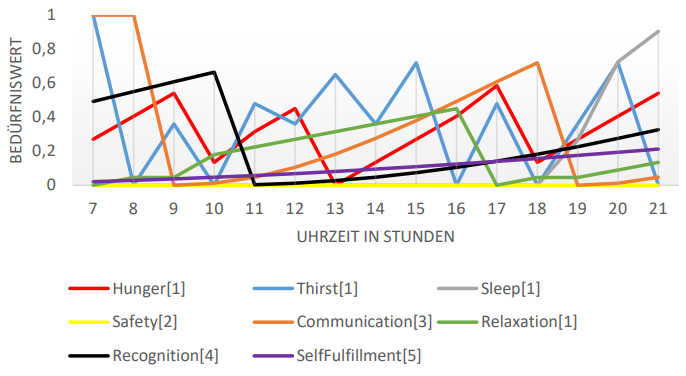
\includegraphics[scale=0.75]{images/schliecker_tagesablauf.PNG}
\caption{Regelbasierter Ansatz, Verlauf der durchschnittlichen Bedürfniswerte}
\label{fig:schliecker_tagesablauf}
\end{figure}

Aus der Verwendung von Regeln ergibt sich theoretisch ein statisches Verhalten, das unter Umständen vorhergesagt werden kann. Da es sich in der Simulation aber um Hintergrundcharaktere mit definierten Aktionen handelt, fallen diese statischen Eigenschaften nicht auf. Da die Bedürfnisse des Agenten nach außen hin nicht sichtbar sind, verhalten sich die Agenten zunächst ähnlich wie die trainierten NPCs. In der Abbildung \ref{fig:rulebased_day_cycle} werden die Verläufe der Bedürfnisse gezeigt, die sich beim regelbasierten Ansatz ergeben. Weiterhin zeigt die Abbildung \ref{fig:action_amounts_manual_vs_ril} einen Vergleich der Häufigkeiten der gewählten Aktionen zum \ac{reinforcement_learning}-Ansatz.

\begin{figure}[H]
\centering
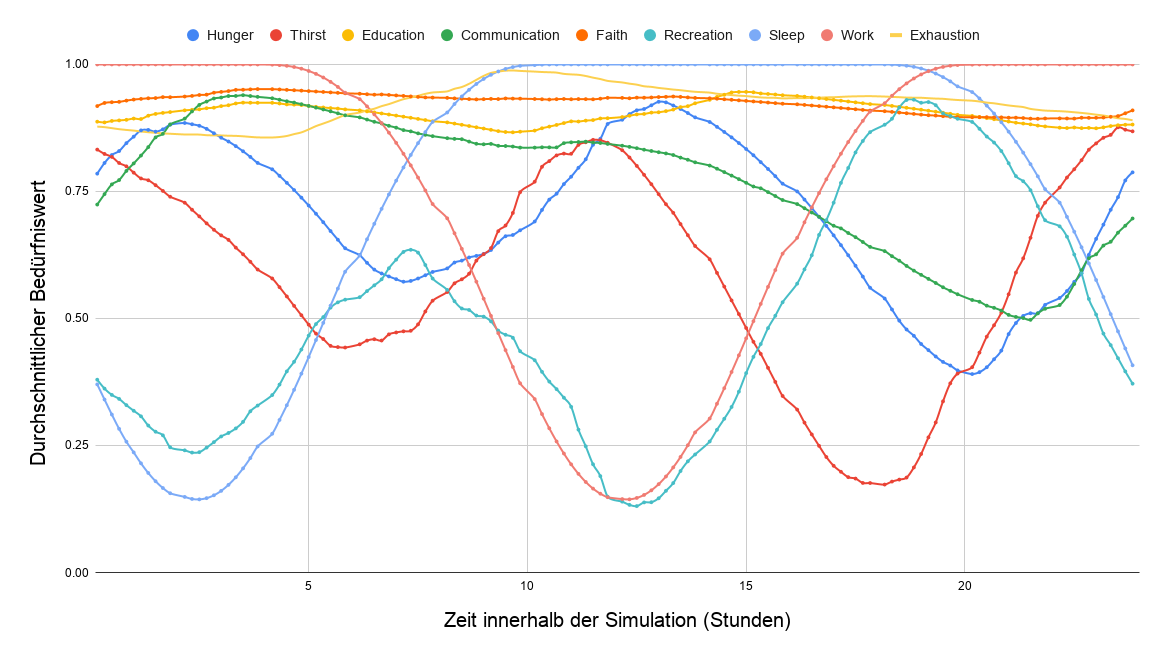
\includegraphics[scale=0.37]{images/rulebased/rulebased_day_cycle.png}
\caption{Regelbasierter Ansatz, Verlauf der durchschnittlichen Bedürfniswerte}
\label{fig:rulebased_day_cycle}
\end{figure}


\begin{figure}[H]
\centering
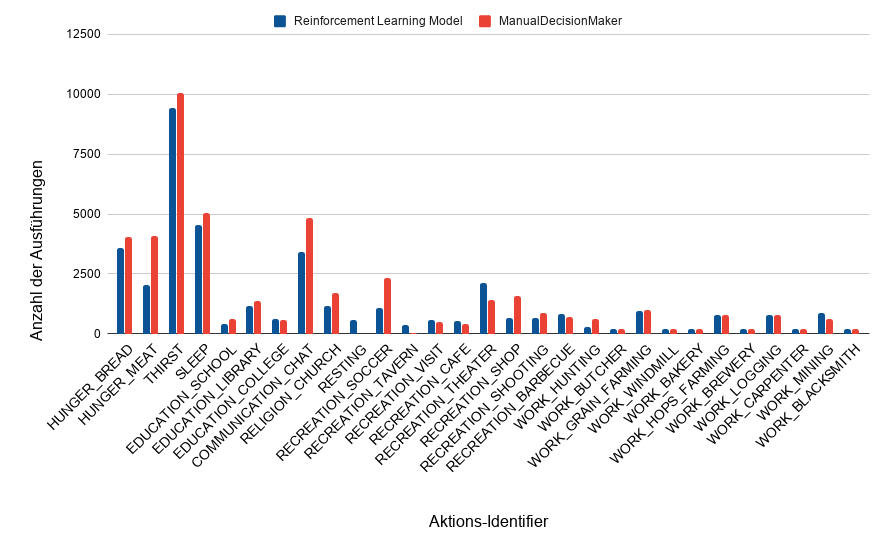
\includegraphics[scale=0.5]{images/training/action_amounts_manual_vs_ril.png}
\caption{Häufigkeiten der Aktionen, regelbasierter Ansatz und ML-Agents-Ansatz}
\label{fig:action_amounts_manual_vs_ril}
\end{figure}

Die beiden Abbildungen zeigen, dass sich insgesamt ein ähnliches Verhalten entwickelt hat. Ein ähnlicher Tagesablauf ist entstanden und die Häufigkeiten der gewählten Aktionen für beide Ansätze weisen hohe Gemeinsamkeiten auf. Erst sobald man einen regelbasierten NPC für einen längeren Zeitraum näher betrachtet, wird klar, dass sein Verhalten durch statische Regeln beeinflusst wird, da Aktionen sofort ausgelöst werden, sobald bestimmte Bedürfniswerte erreicht wurden. In einem realen Spiel kennt der Spieler die Bedürfnisse der Agenten jedoch nicht. Weiterhin handelt es sich hier um Hintergrundcharaktere. In der Regel würde ein Spieler keine Hintergrundcharaktere für eine so lange Zeit beobachten, dass ihm dieses statische Verhalten aufhalten könnte. Der Vorteil aus der Nutzung von Reinforcement Learning ist in diesem Fall also limitiert, da auch ein regelbasierter Ansatz zu einem akzeptablen Ergebnis führt. Der größte Vorteil ergibt sich vielmehr aus der Tatsache, dass die Agenten Entscheidungen aufgrund von sich verändernden Bedürfnissen treffen, die wiederum eine Auswirkung auf die Bedürfnisse des Agenten haben. Dadurch wird glaubwürdig das menschliche Verhalten imitiert.
Die Nutzung von Reinforcement Learning bietet jedoch Vorteile über das eigentliche Verhalten der Agenten hinaus an. Zwar ist der Ansatz mit einem höheren initialen Aufwand verbunden, doch resultiert daraus ein Verfahren, das sehr gut erweiterbar ist. Da der Trainingsvorgang die Auswahl von Aktionen übernimmt, können nun leicht neue Aktionen und Bedürfnisse hinzugefügt werden. Der initiale Aufwand für die Erzeugung eines regelbasierten Ansatzes ist geringer, allerdings ist dabei eine geringere Erweiterbarkeit gegeben. Je mehr Regeln definiert werden müssen, desto höher ist zudem die Wahrscheinlichkeit, dass Regeln sich widersprechen oder durch die hohe Anzahl Fehler im Programmcode eingebaut werden. Weiterhin muss stets eine Priorisierung von Bedürfnissen vorgenommen werden, was im \ac{reinforcement_learning}-Prozess automatisiert und intrinsisch passiert. Der Lernvorgang übernimmt in gewisser Weise die beim \ac{reinforcement_learning}-Ansatz die Definition der Regeln.


Für beide verwendete Ansätze ergibt sich eine hohe Skalierbarkeit, da Entscheidungen pro Agent in einem Abstand von mehreren Sekunden getroffen werden müssen. Die zusätzlich erforderliche Leistung der Nutzung einer höheren Anzahl von Agenten ist daher überschaubar. In einem Test wurden bis zu 1.000 Agenten innerhalb des Dorfes verwendet, die zwar die Kapazitätsgrenzen der Gebäude in der Stadt deutlich überschreiten, aber ohne drastische Performanceverluste dargestellt werden können. 
